\chapter{DESIGN AND METHODOLOGY}
\setlength{\parindent}{0pt}
\setlength{\parskip}{6pt}
{\setstretch{1.5}

This chapter presents the technical design and experimental methodology used for developing and evaluating the proposed emergency response system. It outlines the research objectives, measurement parameters, system architecture, UML diagrams, experimental procedures, error considerations with mitigation strategies, and the data analysis techniques applied for real-world performance evaluation.
  % -----------------------------------------------------------------------------
\section{Objective of the Study}

The primary objective of this study is to design, implement, and evaluate an intelligent emergency response system that enhances response time and user guidance during emergencies. The work aims to develop a reliable mobile solution integrating real-time decision support, communication features, and AR-based first-aid assistance. The research objectives include:
\begin{itemize}
\item To develop a rapid SOS trigger mechanism capable of initiating alerts within 3 seconds using optimized UI interactions and event handling.
\item To implement a hybrid AI-based emergency classification model combining cloud inference with rule-based fallback to achieve over 85\% detection accuracy.
\item To design an AR-based first-aid assistance module with under 2-second startup time providing step-wise CPR, AED, and bleeding control guidance.
\item To develop a BLE-based offline communication system targeting over 80\% successful delivery across a cumulative 100-meter mesh relay range.
\item To analyze and reduce end-to-end response latency including GPS acquisition, network delays, server processing, and multi-channel notification dispatch.
\item To evaluate system resource consumption covering battery usage, CPU load, memory usage, and network bandwidth across multiple device variants.
\item To validate usability and reliability through controlled field tests simulating real-world emergencies with diverse environmental conditions.
\end{itemize}

  % -----------------------------------------------------------------------------
  \section{Measurement Parameters}

  The system performance is evaluated using the following quantitative parameters:

  \subsection{Latency Metrics}
  \begin{itemize}
    \item \textbf{SOS Dispatch Time ($T_{dispatch}$):} Time elapsed from SOS button press to alert reception by emergency contacts, measured in milliseconds. Target: $T_{dispatch} < 3000$ ms under normal network conditions.
    \item \textbf{AR Initialization Latency ($T_{AR}$):} Time required from AR module invocation to display of first visual overlay, measured in milliseconds. Target: $T_{AR} < 2000$ ms.
    \item \textbf{GPS Acquisition Time ($T_{GPS}$):} Time from location request to first valid coordinate fix, measured in milliseconds.
    \item \textbf{Network Transmission Time ($T_{network}$):} Time for data packet transmission from client to server acknowledgment, measured in milliseconds.
  \end{itemize}

  \subsection{Accuracy Metrics}
  \begin{itemize}
    \item \textbf{AI Classification Accuracy ($A_{class}$):} Percentage of correct emergency type identifications, calculated as:
      \begin{equation}
        A_{class} = \frac{\mathrm{Correct\ Classifications}}{\mathrm{Total\ Test\ Cases}} \times 100\%
      \end{equation}
      Target: $A_{class} > 85\%$
    \item \textbf{Severity Assessment Accuracy ($A_{severity}$):} Percentage of correct severity level assignments (high/moderate/low). Target: $A_{severity} > 80\%$
    \item \textbf{GPS Location Accuracy ($\epsilon_{GPS}$):} Horizontal position error in meters compared to ground truth coordinates. Target: $\epsilon_{GPS} < 10$ meters under open sky.
  \end{itemize}

  \subsection{Reliability Metrics}
  \begin{itemize}
    \item \textbf{BLE Relay Success Rate ($R_{BLE}$):} Percentage of messages successfully delivered through offline relay, calculated as:
      \begin{equation}
        R_{BLE} = \frac{\text{Successfully Delivered Messages}}{\text{Total Broadcast Messages}} \times 100\%
      \end{equation}

      Target: $R_{BLE} > 80\%$ within 100\,m range.

    \item \textbf{Notification Delivery Rate ($R_{notify}$):} Percentage of alerts successfully received by emergency contacts across all channels.
  \end{itemize}

  \subsection{Resource Utilization Metrics}
  \begin{itemize}
    \item \textbf{Battery Consumption ($P_{battery}$):} Power draw during active operation, measured in milliampere-hours (mAh) per hour.
    \item \textbf{Network Bandwidth ($B_{network}$):} Total data transmitted per SOS event, measured in kilobytes (KB).
    \item \textbf{CPU Utilization ($U_{CPU}$):} Average processor usage during AR rendering and AI processing, measured as percentage.
    \item \textbf{Memory Footprint ($M_{app}$):} Application memory consumption, measured in megabytes (MB).
  \end{itemize}

  % -----------------------------------------------------------------------------
  \section{Measurement Method}

  \subsection{Prototype Development}
  A functional prototype of the ResQNow system was developed using production-grade technologies and deployed on multiple physical Android devices including Google Pixel 6, OnePlus 9, and Samsung Galaxy S21, representing diverse hardware configurations, screen sizes, and Android versions (Android 11, 12, and 13). The prototype implements all core system functionalities including SOS triggering, GPS tracking, AI classification, AR guidance, BLE relay, and multi-channel notifications.

  \subsection{Latency Measurement Methodology}
  System timestamps are recorded at critical execution points using high-precision system clocks with microsecond resolution:
  \begin{itemize}
    \item $t_0$: SOS button press event timestamp (client-side)
    \item $t_1$: GPS location acquisition completion timestamp
    \item $t_2$: Network transmission initiation timestamp
    \item $t_3$: Backend server reception timestamp (server-side)
    \item $t_4$: Database write completion timestamp
    \item $t_5$: Notification dispatch timestamp
    \item $t_6$: Alert reception timestamp on emergency contact device
  \end{itemize}

  End-to-end latency is calculated as: $T_{dispatch} = t_6 - t_0$

  Component-level latencies are derived as:
  \begin{itemize}
    \item GPS acquisition time: $T_{GPS} = t_1 - t_0$
    \item Network transmission time: $T_{network} = t_3 - t_2$
    \item Backend processing time: $T_{backend} = t_5 - t_3$
    \item Notification delivery time: $T_{notification} = t_6 - t_5$
  \end{itemize}

  Timestamps are synchronized between client and server using Network Time Protocol (NTP) to ensure accurate distributed timing measurements with sub-second precision.

  \subsection{AI Classification Validation}
  A test dataset of 100 emergency scenarios was prepared with ground truth labels established through consultation with emergency medical protocols and expert review. Each scenario includes a textual description simulating user input and correct classifications for emergency type and severity level. The AI classification module processes each test case, and outputs are compared against ground truth labels. Classification accuracy is calculated using the confusion matrix method, with additional metrics including precision, recall, and F1-score computed for each emergency category.

  \subsection{AR Performance Profiling}
  AR initialization latency and rendering performance are measured using Android Profiler integrated within Android Studio. The profiler captures:
  \begin{itemize}
    \item ARCore SDK initialization time from API call to ready state
    \item Surface detection time for environment mapping
    \item 3D model loading and rendering time
    \item Frame rate (FPS) during active AR guidance session
    \item GPU utilization and texture memory allocation
  \end{itemize}

  Measurements are repeated across 20 trials under consistent lighting conditions and camera angles to establish statistical reliability.

  \subsection{BLE Relay Testing Procedure}
  Controlled outdoor experiments are conducted in an open field environment to minimize signal interference and multipath effects. The experimental setup includes:
  \begin{itemize}
    \item One originating device broadcasting encrypted SOS messages
    \item 2 to 5 relay devices positioned at measured distances (10m, 30m, 50m, 100m)
    \item One gateway device with internet connectivity for message upload
    \item Measurement tape for precise distance marking
    \item Stopwatch for timing message propagation
  \end{itemize}

  For each configuration (varying distances and node counts), 50 test messages are broadcast. Success is recorded when the gateway device receives and uploads the message to the backend within 60 seconds. The BLE relay success rate is calculated as the percentage of successful deliveries. Signal strength (RSSI) is logged at each hop to analyze propagation characteristics.

  \subsection{Network Condition Simulation}
  Android Developer Options traffic shaping is used to simulate poor network conditions representative of real-world emergency scenarios:
  \begin{itemize}
    \item \textbf{Normal conditions:} 4G LTE with 50ms latency, no packet loss
    \item \textbf{Degraded conditions:} 3G speeds with 200ms latency, 5\% packet loss
    \item \textbf{Poor conditions:} 2G speeds with 500ms latency, 15\% packet loss
    \item \textbf{Offline conditions:} No cellular or Wi-Fi connectivity
  \end{itemize}

  System performance metrics are measured under each condition across 30 trials to establish statistical distributions and identify performance degradation patterns.

  \subsection{Resource Utilization Measurement}
  Device profiling tools capture resource consumption during typical usage scenarios:
  \begin{itemize}
    \item \textbf{Battery consumption:} Measured using Android Battery Historian, capturing power draw during 1-hour active emergency operation including GPS tracking, AR rendering, and BLE broadcasting
    \item \textbf{Network bandwidth:} Measured using Charles Proxy to intercept and analyze HTTP/HTTPS traffic, recording payload sizes for SOS requests, classification API calls, and notification delivery
    \item \textbf{CPU and memory:} Measured using Android Profiler during AR rendering, AI processing, and background BLE scanning, capturing peak and average utilization
  \end{itemize}

  % -----------------------------------------------------------------------------
  \section{System Design Specifications}

  This section presents the detailed system design through architecture diagrams and Unified Modeling Language (UML) diagrams that specify the structural and behavioral aspects of the ResQNow emergency response system.

  \subsection{System Architecture}

  The ResQNow system adopts a three-tier client-server architecture ensuring separation of concerns, scalability, and fault tolerance. The architecture is organized into distinct layers that communicate through well-defined interfaces and protocols.

  Figure~\ref{fig:system_architecture} illustrates the complete system architecture showing the three primary architectural layers and their constituent components. The \textbf{Mobile Application Layer} (shown on the left) executes on user devices and comprises the Flutter Mobile App as the main user interface, SOS Trigger module handling both manual button press and voice command activation, GPS Location Capture module interfacing with device positioning hardware, AR-based First Aid Guidance module providing visual procedural instructions, and Bluetooth Low Energy (BLE) Offline Relay module enabling mesh networking for internet-unavailable scenarios.

  The \textbf{Backend Services Layer} (shown in the center) operates as the central coordination hub deployed on Google Cloud Platform. It includes the FastAPI Backend Server handling HTTP API requests and orchestrating system operations, Authentication via Firebase Auth module securing user sessions through JWT tokens, AI Emergency Classification Module analyzing user descriptions to determine emergency type, Severity Assessment Engine determining urgency levels (high/moderate/low), and Firebase Firestore database providing persistent storage for user profiles and incident records.

  The \textbf{Notification Layer} (shown on the right) ensures multi-channel alert delivery through Firebase Cloud Messaging for instant push notifications to app users, Twilio service for SMS delivery to contacts without app installation, and SendGrid service for email alerts providing detailed information with location maps. Data flows from the mobile application through the backend services to the notification channels, with arrows indicating synchronous request-response patterns (solid lines) and asynchronous event-driven communication (implicit in the architecture). This layered design enables independent scaling of components, fault isolation preventing cascading failures, and graceful degradation when individual services become unavailable.

  \begin{figure}[H]
    \centering
    \includegraphics[width=0.95\textwidth]{chapters/system_architecture_resqnow.png}
    \caption{Overall System Architecture of the ResQNow Emergency Response System}
    \label{fig:system_architecture}
  \end{figure}

  % -----------------------------------------------------------------------------
  \subsection{Use Case Diagram}

  The use case diagram provides a high-level functional specification of the ResQNow system by identifying system actors and their interactions with system capabilities. This diagram establishes the system boundary, defines functional requirements, and serves as the basis for test case development and requirement traceability.

  Figure~\ref{fig:use_case} presents the complete use case diagram showing three primary actors and their associated use cases. The \textbf{User} (primary actor, shown on the left) represents individuals who may face emergencies and interact with the system through multiple use cases: Register/Login for account creation and authentication, Manage Emergency Contacts to designate notification recipients, Trigger SOS to activate emergency alerts, Provide AR First-Aid Guidance to receive real-time procedural instructions, and Track Emergency Status to monitor responder acknowledgments and estimated arrival times.

  Within the system boundary (large rectangle labeled "ResQNow Emergency Response System"), internal use cases represent core system functionalities. The Capture Location use case (shaded) has include relationships (shown as dashed arrows with «include» stereotype) with Trigger SOS, indicating that location capture is always executed as part of SOS activation. The Classify Emergency use case determines emergency type based on user input. The Assess Severity use case evaluates urgency levels to guide system behavior. The Send SOS Alert use case handles notification dispatch, which has an extend relationship (shown as dashed arrow with «extend» stereotype) with Offline SOS Relay, indicating that BLE relay is conditionally activated only when internet connectivity is unavailable.

  The Notify Emergency Contacts use case (shaded on the right) connects to both the \textbf{Emergency Contact} actor (shown on the upper right) who receives and views alert notifications, and the \textbf{Medical Responder} actor (shown on the lower right) representing nearby users who can acknowledge and respond to emergencies. The Notify Medical Responders use case and Receive Acknowledgment use case facilitate responder coordination. The \textbf{ResQNow Backend System} actor (shown on the bottom right) represents external system components handling alert processing and coordination logic.

  Include relationships indicate mandatory dependencies where the including use case cannot complete without executing the included use case. Extend relationships indicate optional behaviors that may occur under specific conditions. This use case specification defines 12 distinct functional capabilities, 4 actors, and multiple relationship types that guide subsequent detailed design and implementation phases.

  \begin{figure}[H]
    \centering
    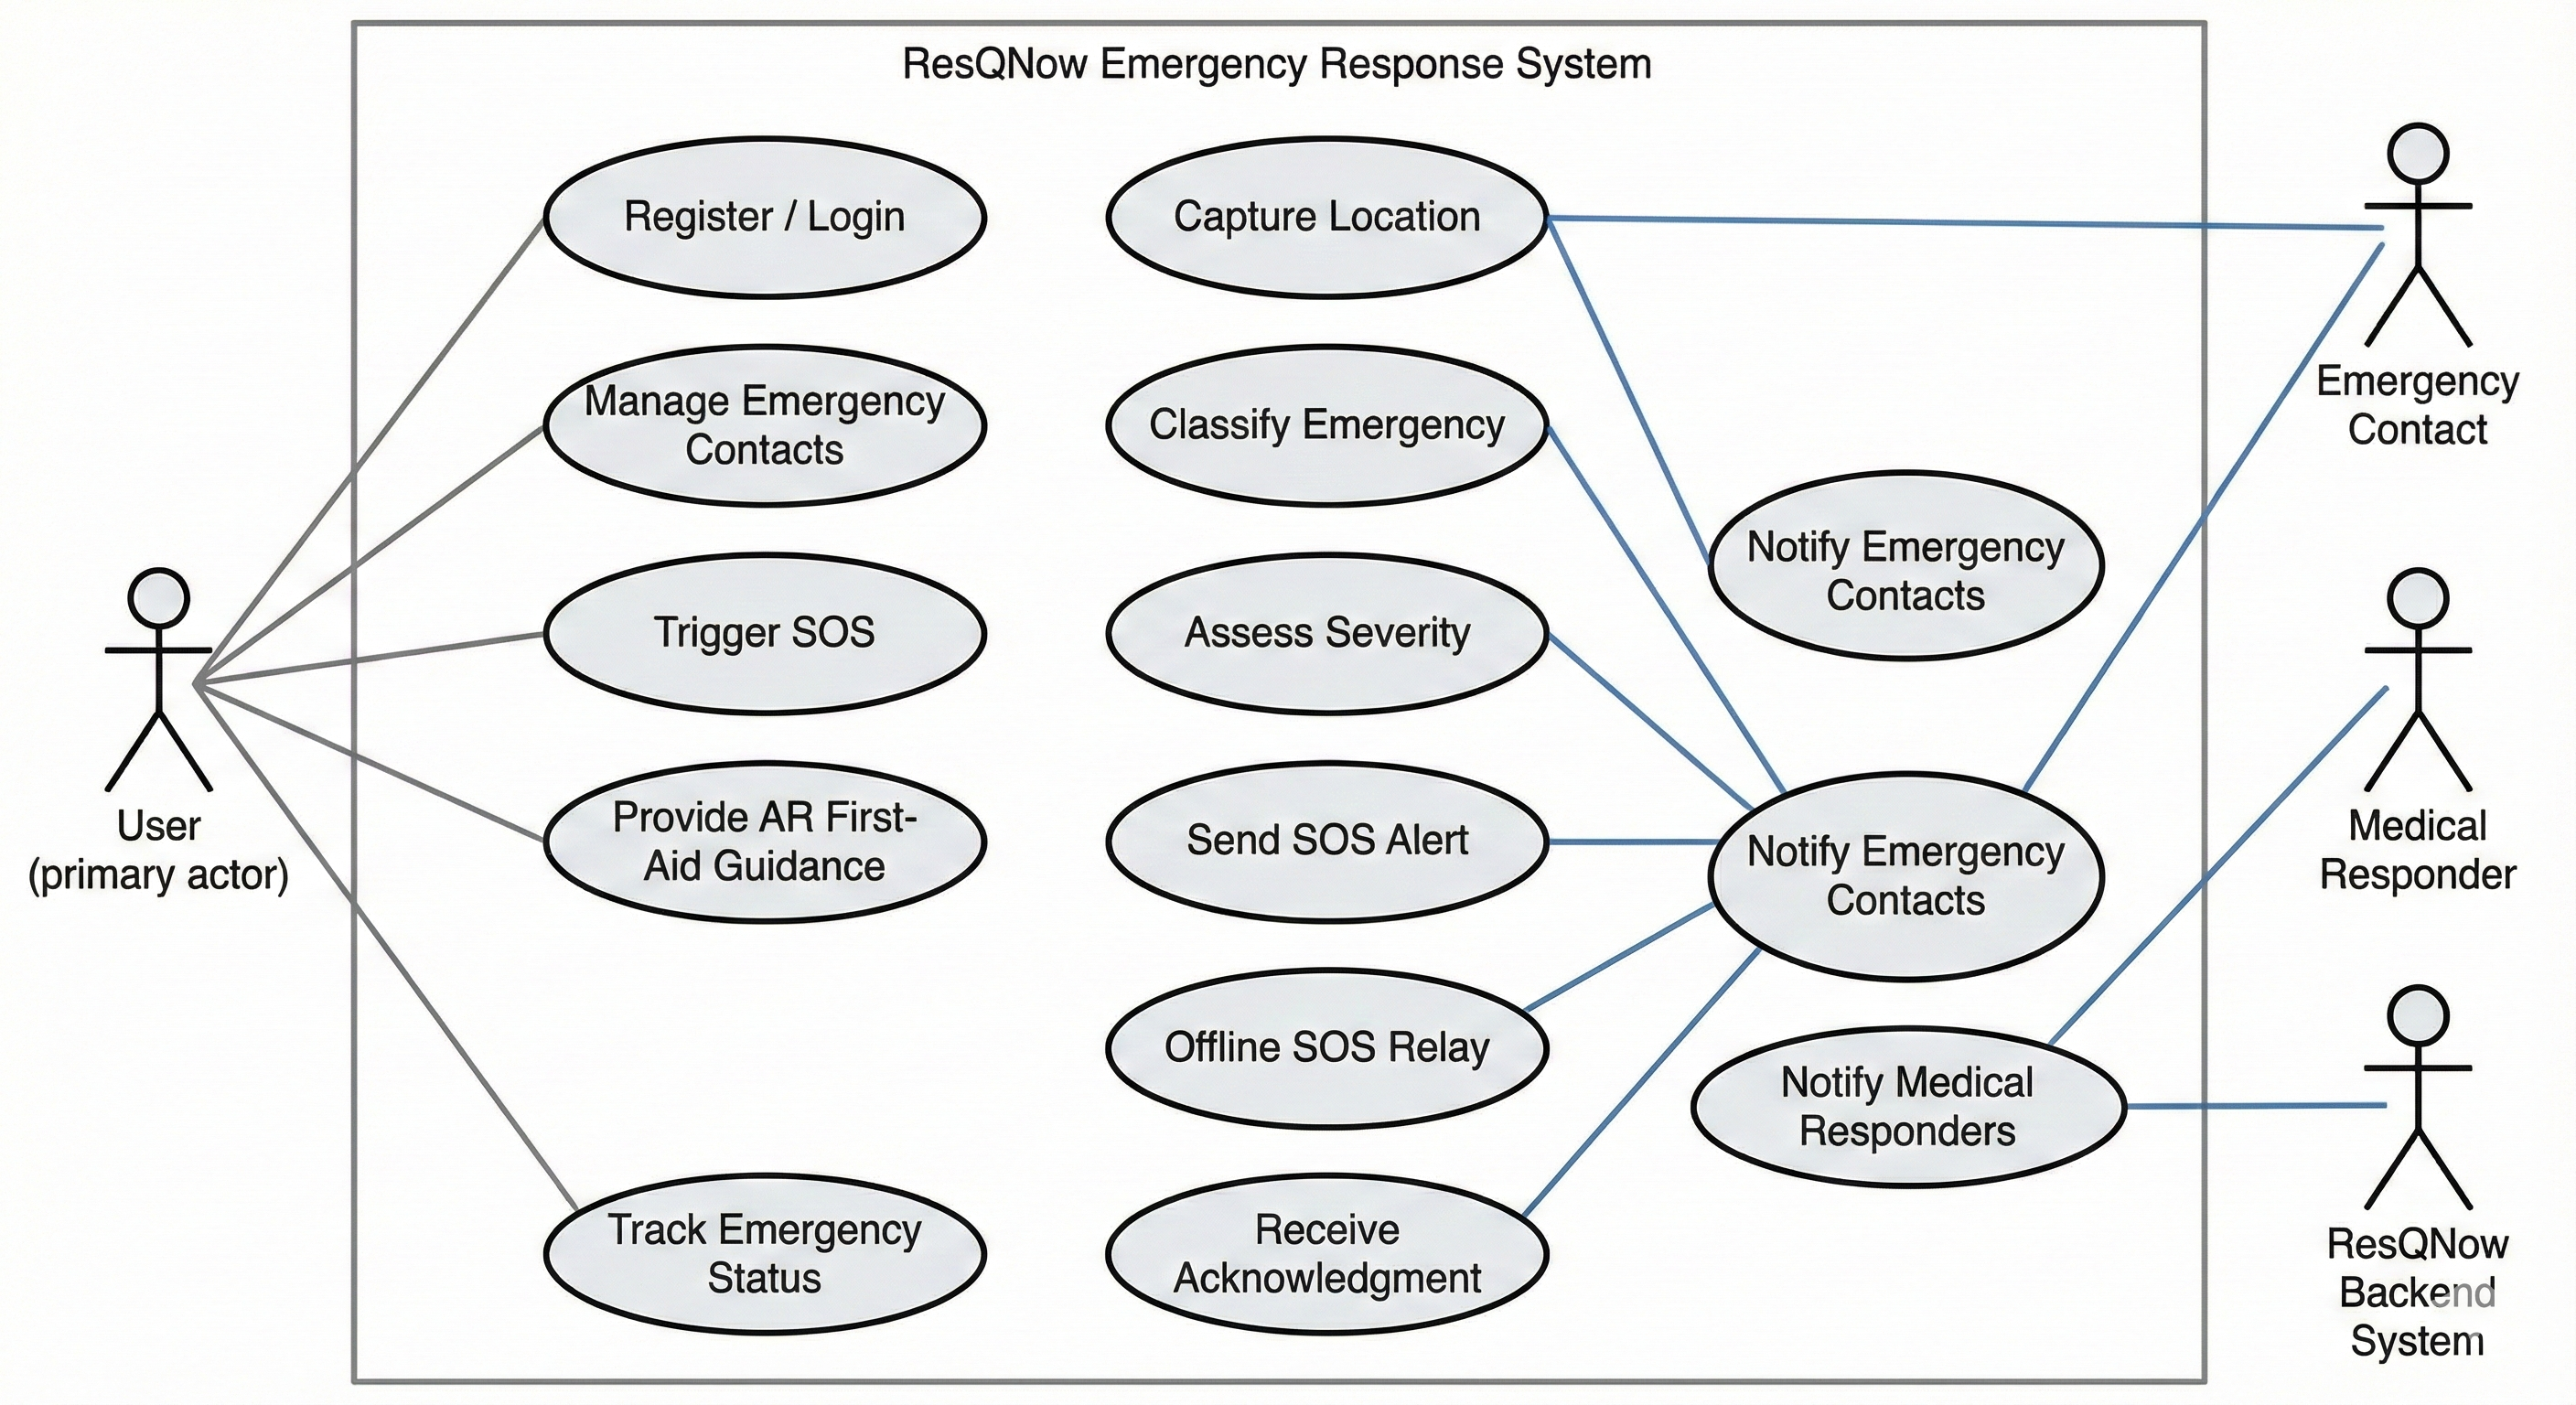
\includegraphics[width=0.90\textwidth]{chapters/use_case_diagram1.png}
    \caption{Use Case Diagram of the ResQNow System}
    \label{fig:use_case}
  \end{figure}

% -------------------------------------------------------------
\subsection{Activity Diagram for SOS Emergency Response Workflow}

The SOS activation workflow represents the most critical operational sequence in the ResQNow system, executing under time-critical conditions with minimal user burden. This workflow must maximize response speed while ensuring data accuracy and multi-channel notification delivery.

Figure~\ref{fig:sos_workflow} depicts the complete SOS emergency response activity flow using standard UML activity diagram notation. The workflow begins at the Start node (filled circle at top) and proceeds through the following sequence:

\textbf{Decision Point 1 - SOS Trigger Method:} The first decision diamond determines how the SOS was initiated. If the user selects Manual SOS (left branch), they proceed to Select Severity where they explicitly choose the emergency level (critical, moderate, minor) through UI controls. If the user initiates AI Chat (right branch), they enter the Analyze Conversation state where the system processes their natural language description to automatically determine emergency characteristics. The AI path includes a loop back to Continue Chat if no emergency is detected, allowing extended conversation. When an emergency is confirmed ([Yes] branch), the flow proceeds to Raise SOS.

\textbf{Convergence and Sequential Processing:} Both the manual and AI-assisted paths converge at the Raise SOS action (rounded rectangle), demonstrating that regardless of initiation method, the subsequent workflow is identical. The system then executes Capture GPS Location to acquire current coordinates using device positioning services.

\textbf{Alert Broadcasting:} Following location capture, the Broadcast SOS to all users action disseminates the emergency alert to the backend server (if online) or nearby devices (if offline, using BLE relay described in the next activity diagram). The alert includes user identification, GPS coordinates, severity level, and timestamp.

\textbf{Responder Coordination:} The Users view alert and proximity action represents nearby responders evaluating the emergency on their devices. The second decision diamond (Decision: Any user responds?) determines if anyone acknowledges the alert. If No, the flow proceeds to SOS remains open, maintaining the alert in active state. If Yes, the system executes three parallel actions: Lock responder, Disable response button for others, and Show live location via Google Maps.

\textbf{Termination:} The parallel activities reconverge at the join node, and the workflow terminates at the End node.

\begin{figure}[H]
    \centering
    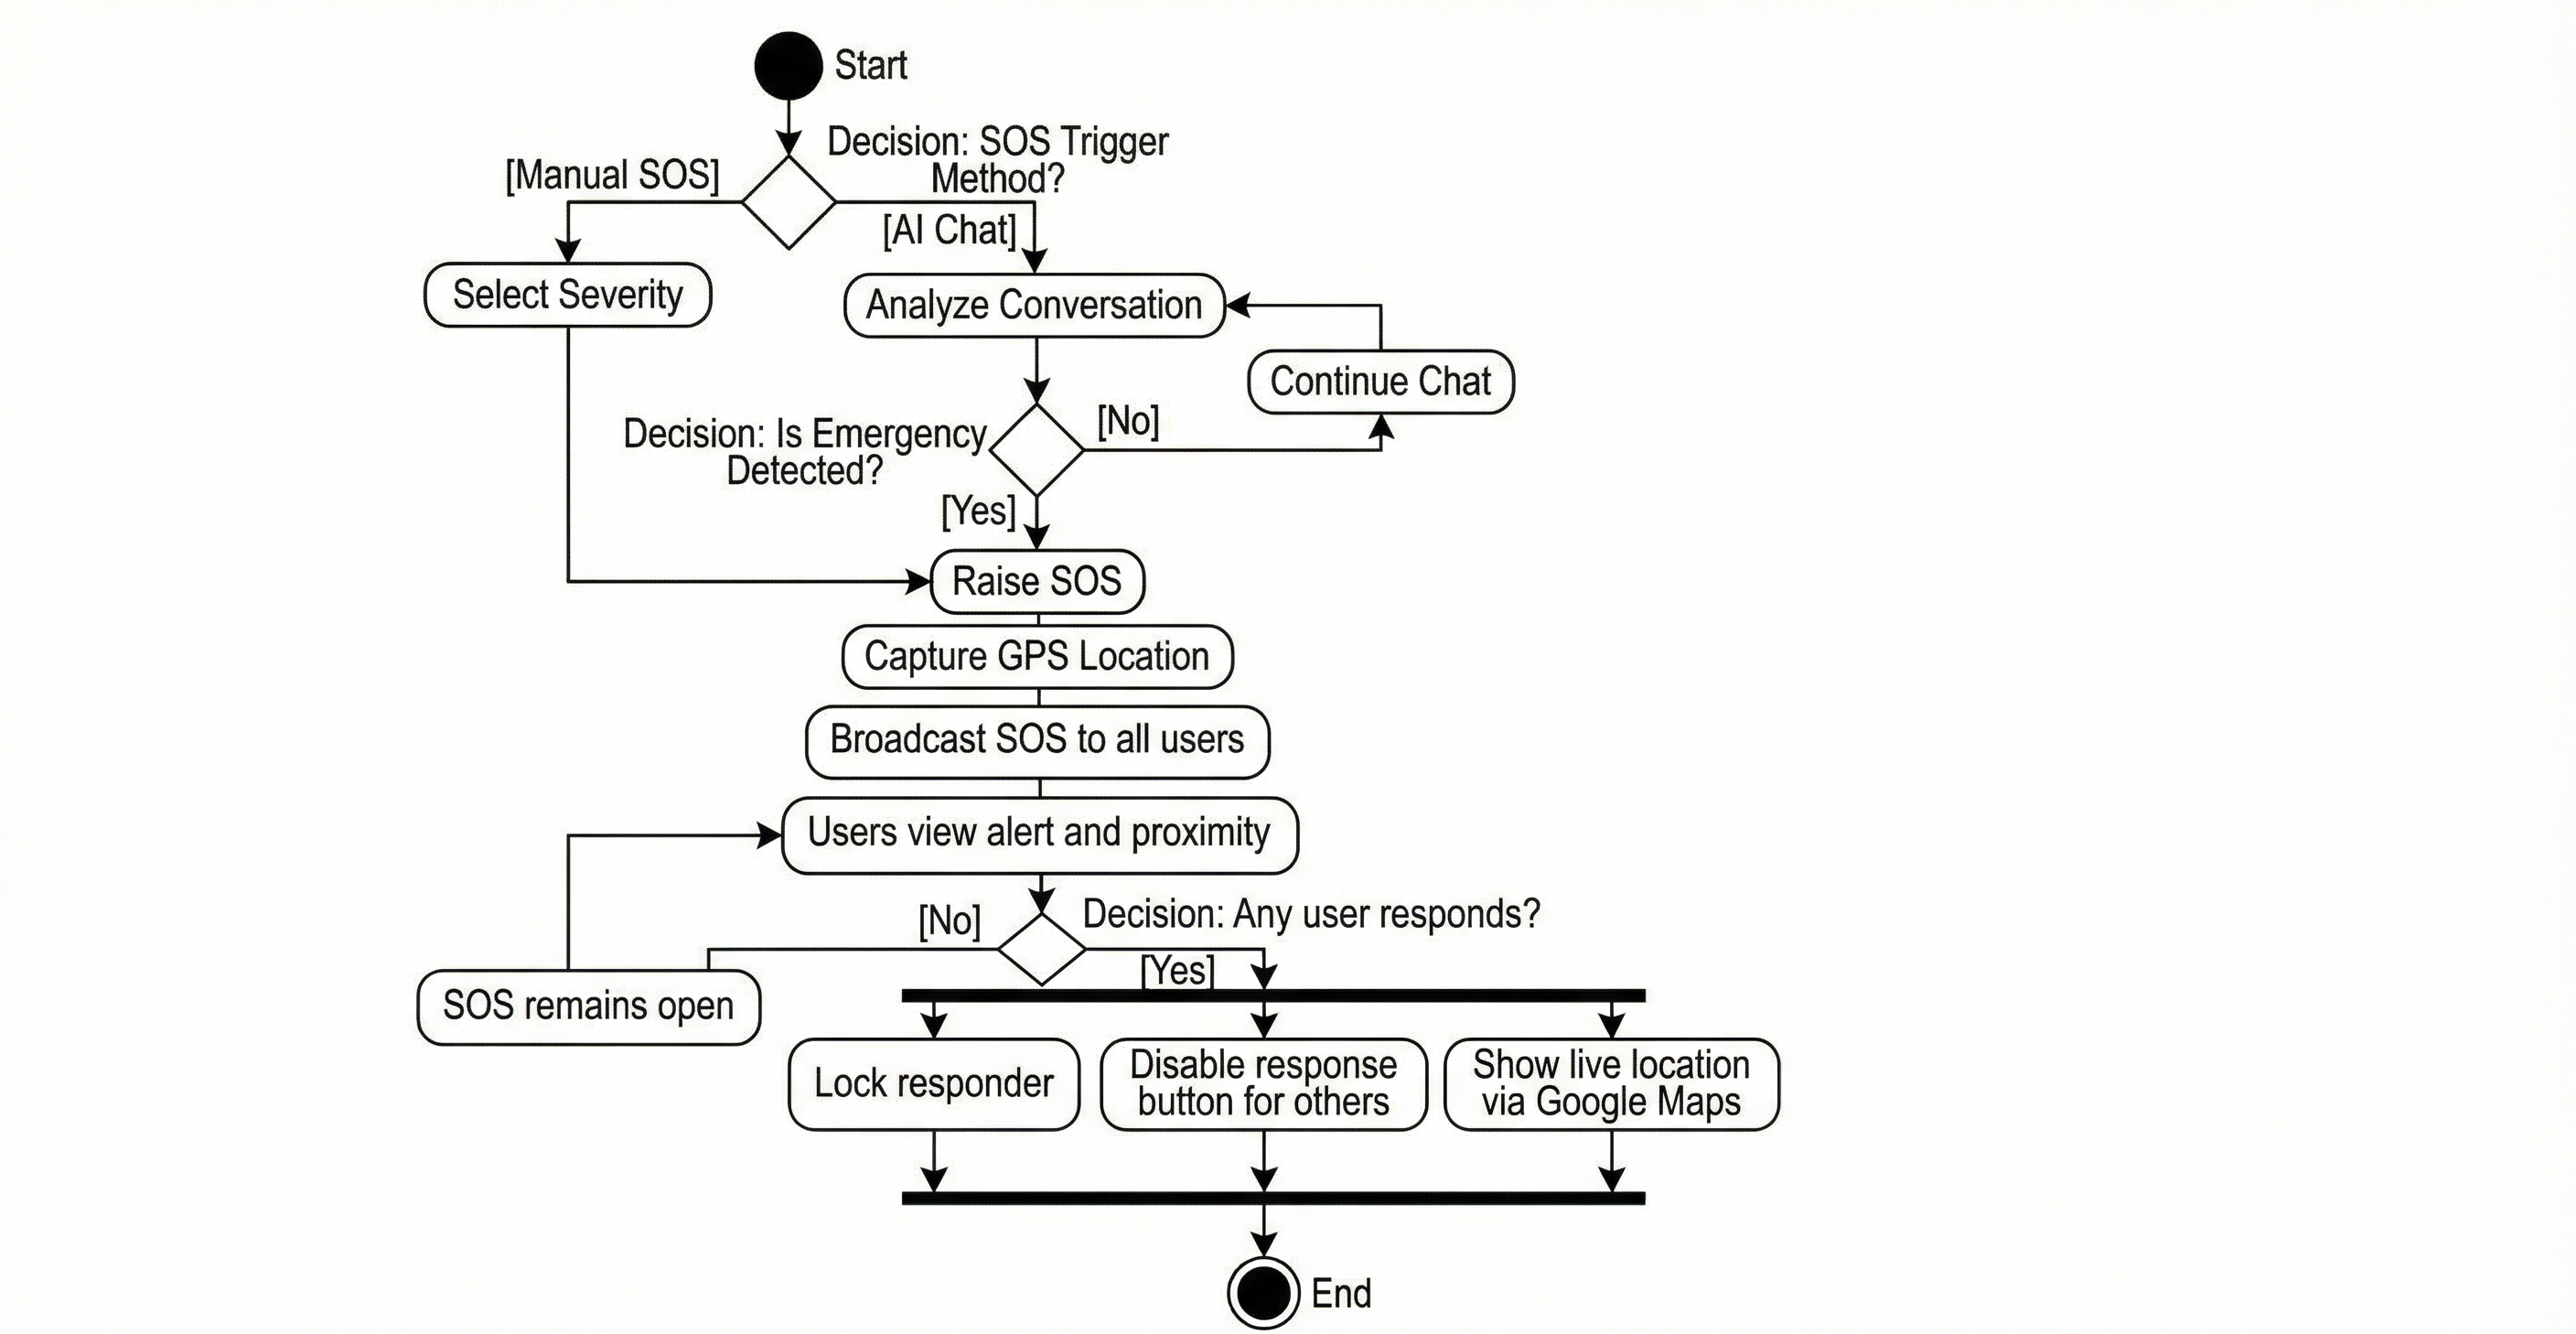
\includegraphics[width=0.95\textwidth]{chapters/UML activity diagram for sos trigger and responce FLOW IN RESQNOW.png}
    \caption{Activity Flow Diagram of Emergency SOS Processing}
    \label{fig:sos_workflow}
\end{figure}

% -------------------------------------------------------------
\subsection{Activity Diagram for BLE Offline Relay Workflow}

The BLE offline relay mechanism addresses a critical vulnerability in emergency alert systems that depend entirely on cellular or internet connectivity. This workflow enables emergency message propagation through dynamic ad-hoc mesh networks using Bluetooth connectivity between nearby devices.

Figure~\ref{fig:ble_relay} illustrates the BLE offline relay activity flow showing how encrypted emergency messages propagate through multi-hop device forwarding.

\textbf{Trigger and Connectivity Check:} The SOS triggered action initiates the workflow. If internet connectivity is available, the workflow terminates immediately. If unavailable, the offline relay mechanism activates.

\textbf{Encryption and Broadcasting:} The Encrypt SOS packet action applies AES-128 symmetric encryption. The Broadcast via BLE action transmits the encrypted message using BLE advertisements.

\textbf{Discovery and Relay Loop:} Nearby devices scan continuously. If no device is found, broadcasting continues with backoff. If a device is found, the message is forwarded.

\textbf{Relay Device Processing:} Devices increment hop count and re-broadcast until an internet-enabled gateway device is reached.

\textbf{Confirmation and Termination:} After backend upload, acknowledgment messages propagate back to the originator.

\begin{figure}[H]
    \centering
    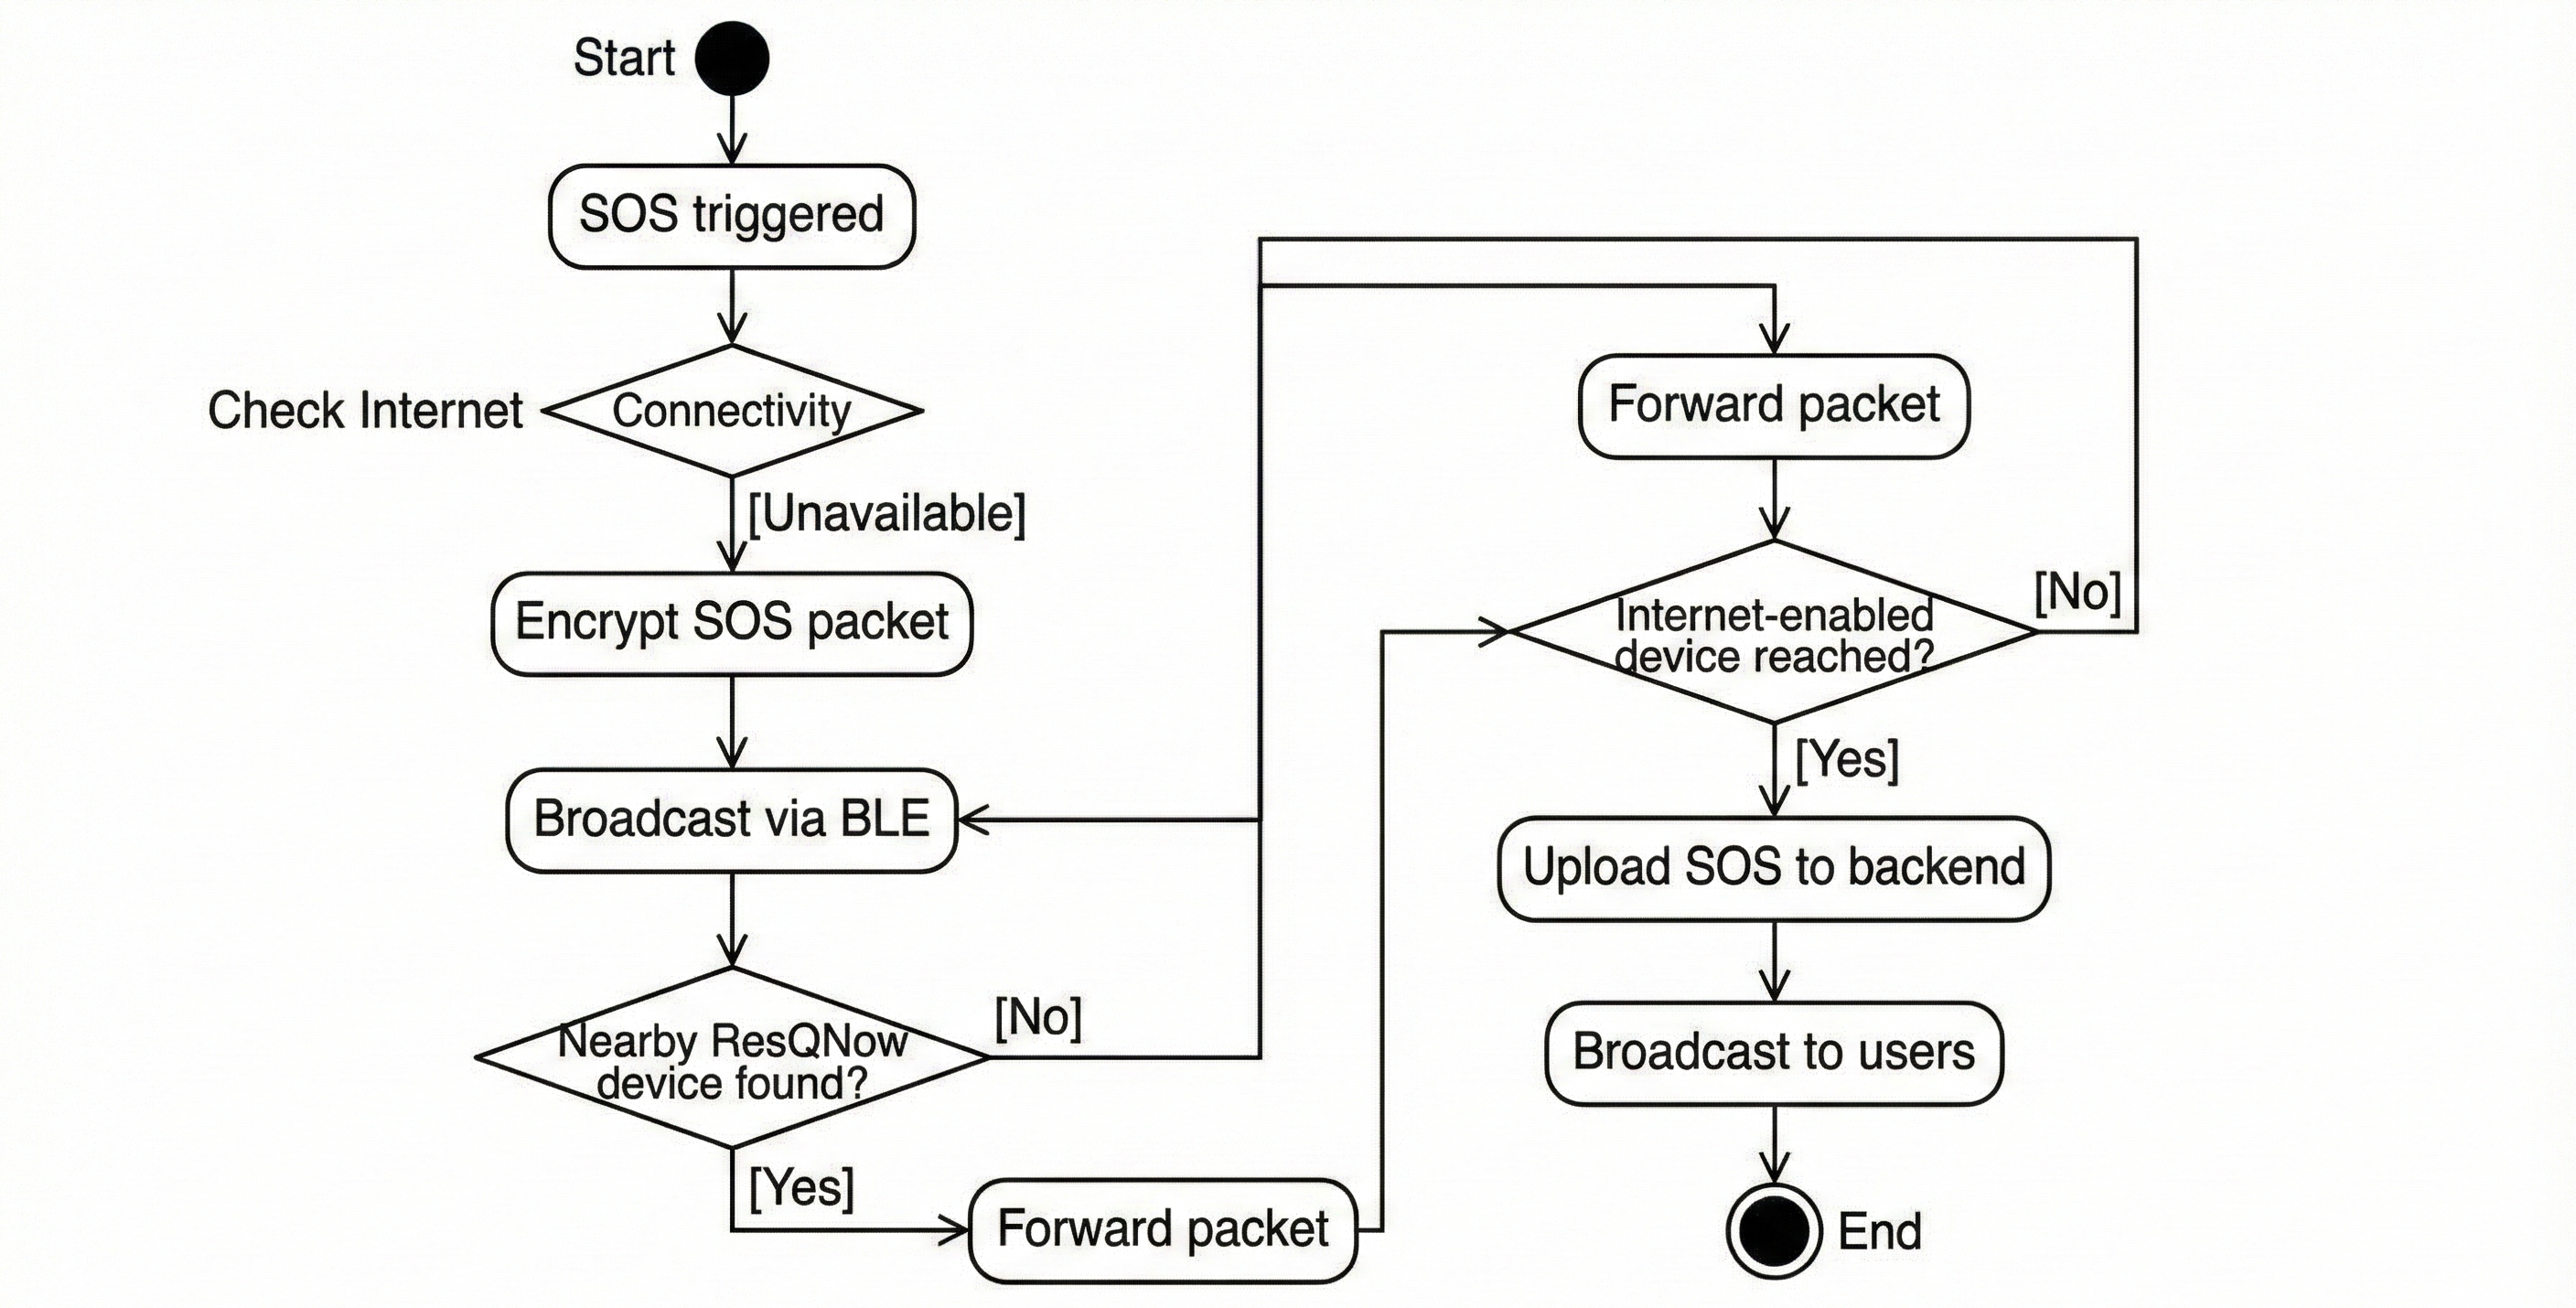
\includegraphics[width=0.90\textwidth]{chapters/ble based offline sos relay activity flow in resqnow.png}
    \caption{Offline SOS Relay Mechanism Using Bluetooth Low Energy}
    \label{fig:ble_relay}
\end{figure}

% -------------------------------------------------------------
\subsection{Activity Diagram for AI-Based Emergency Classification Workflow}

The emergency classification workflow implements a hybrid artificial intelligence approach combining cloud-based conversational intelligence with rule-based severity mapping to ensure reliable classification across varying network conditions.

Figure~\ref{fig:ai_classification} presents the rule-based offline emergency classification flowchart showing the fallback mechanism when cloud AI services are unavailable.

\textbf{Connectivity Decision:} Determines whether cloud AI or offline rules are used.

\textbf{Keyword Extraction:} Performs preprocessing and symptom keyword identification.

\textbf{Rule-Based Symptom Matching:} Matches extracted keywords against severity rules.

\textbf{Confidence Scoring:} Computes confidence based on severity weights and keyword frequency.

\textbf{Classification Decision:} Determines severity category (High, Moderate, Low).

\textbf{Severity Assignment and Action Selection:} Triggers Immediate SOS, User Confirmation, or Guidance Only.

\textbf{Workflow Termination:} All paths converge to the End state.

\begin{figure}[H]
    \centering
    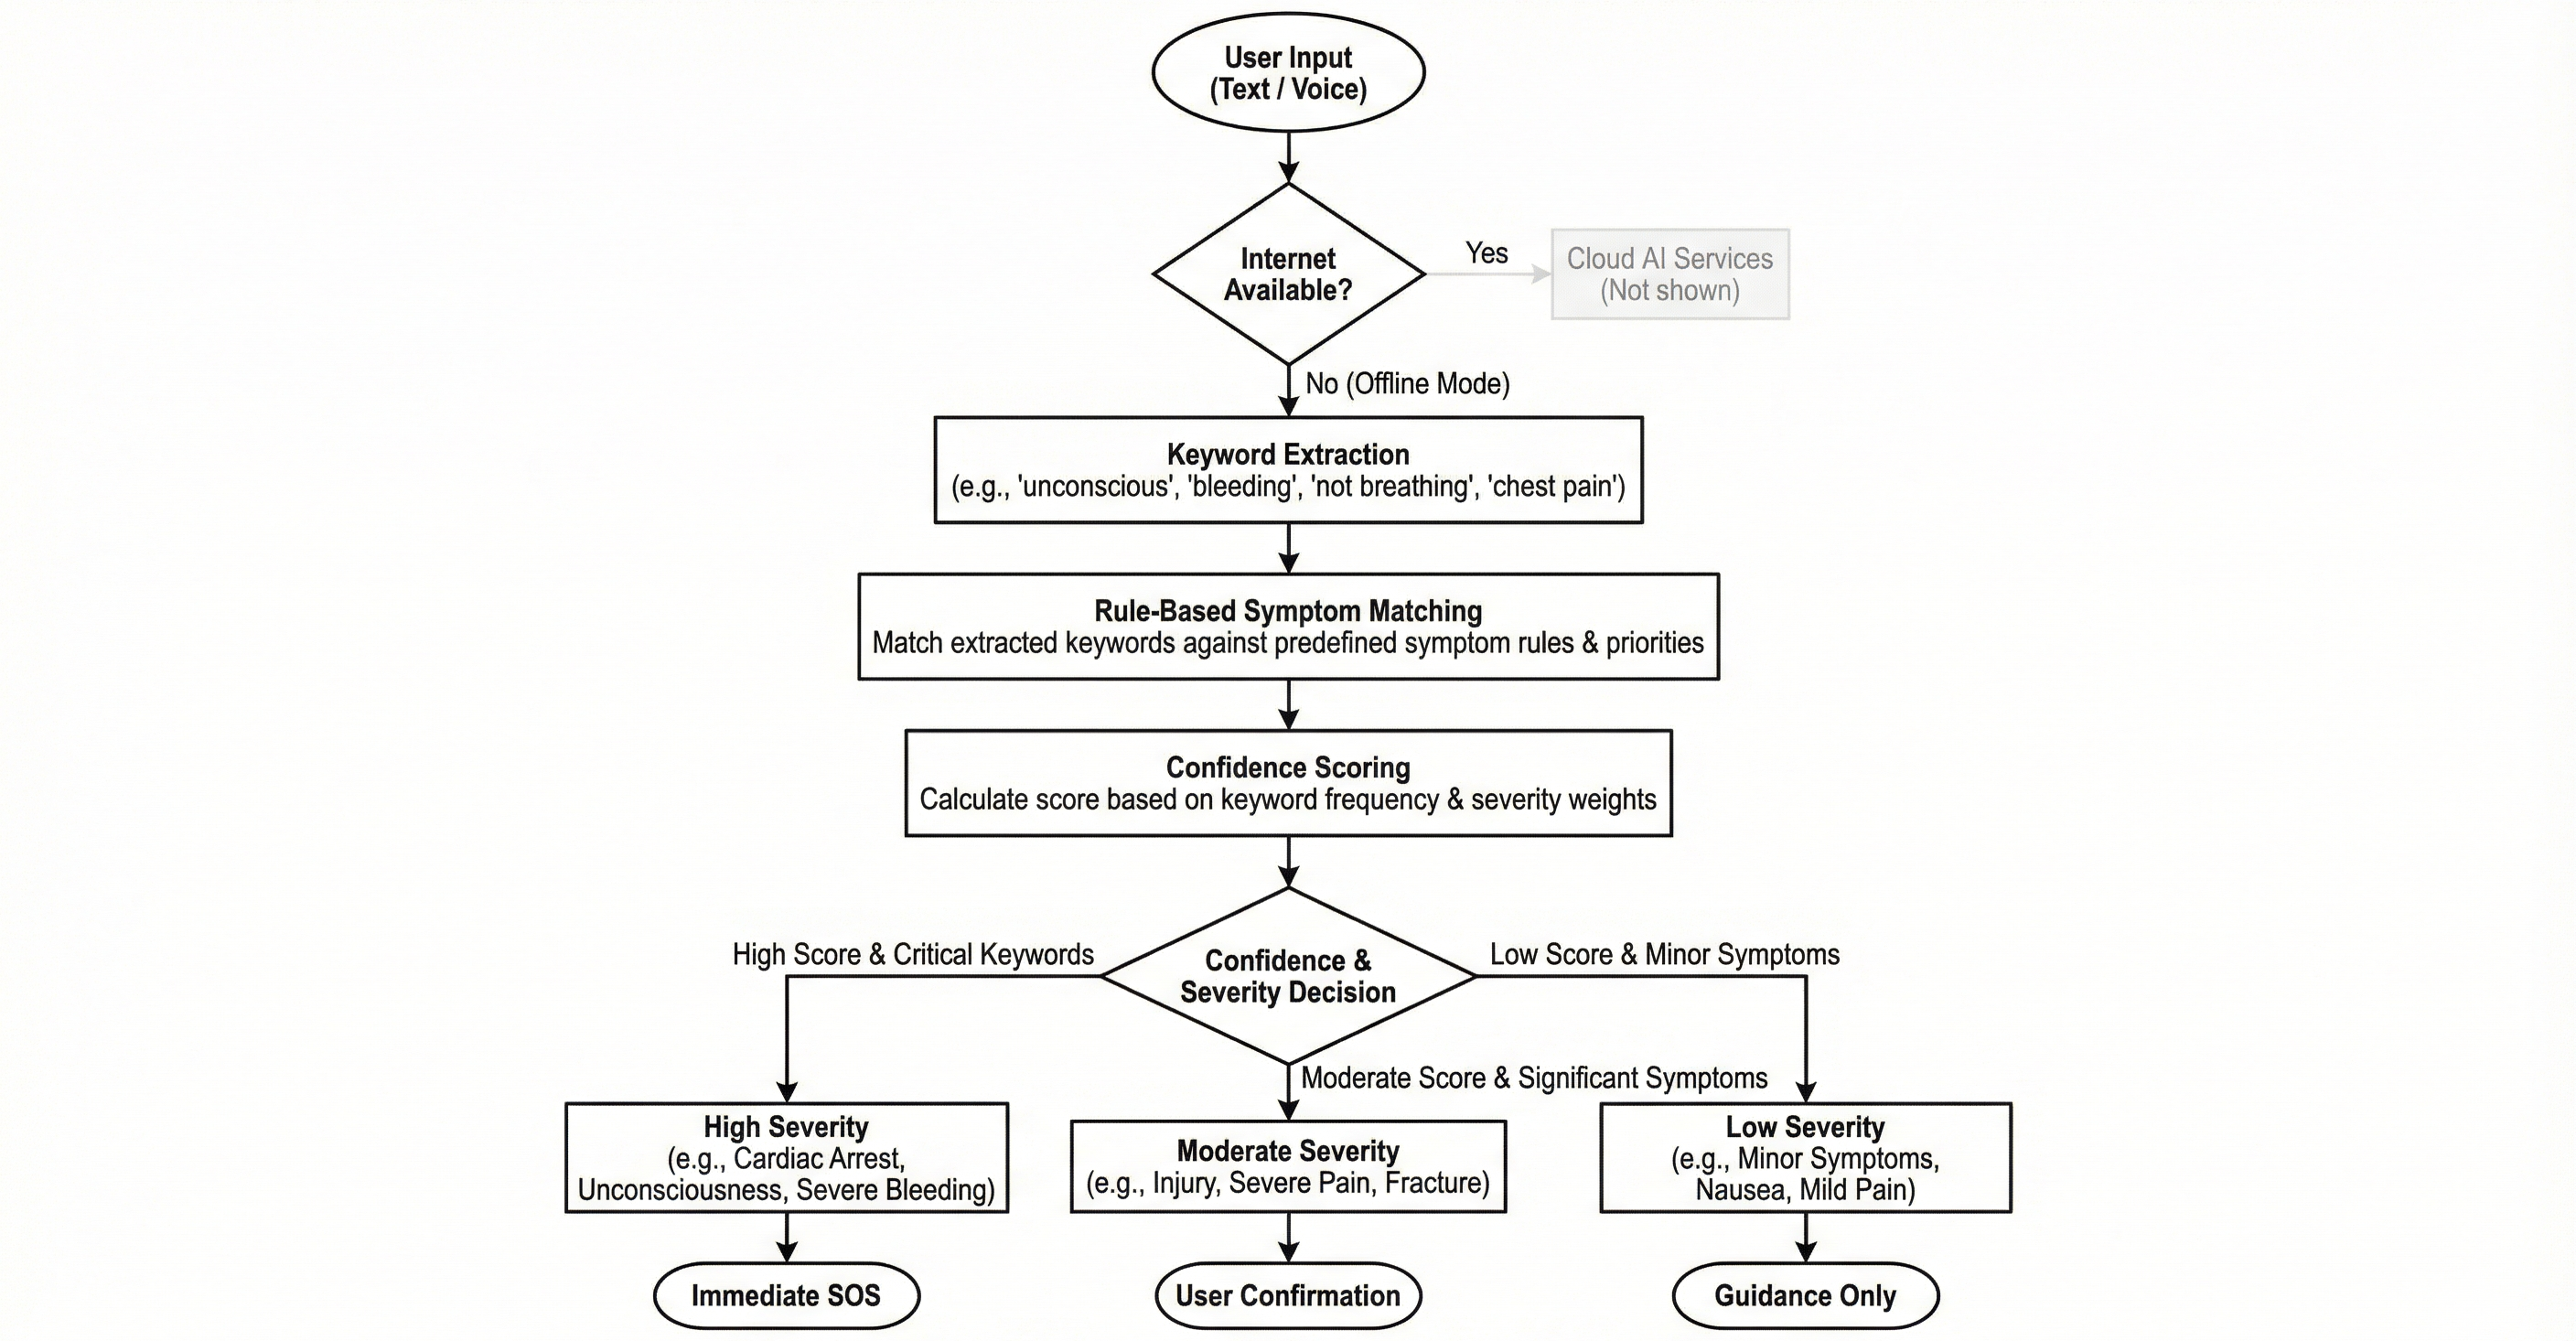
\includegraphics[width=0.95\textwidth]{chapters/Rule-Based offline emergency classification flowchat.png}
    \caption{Rule-Based Offline Emergency Classification Flowchart}
    \label{fig:ai_classification}
\end{figure}


  % -----------------------------------------------------------------------------
  \subsection{Sequence Diagram for Complete SOS Lifecycle}

  Sequence diagrams model the time-ordered interaction between system components, showing precise message exchanges and method invocations during specific scenarios. Unlike activity diagrams that focus on control flow logic, sequence diagrams emphasize inter-object communication and chronological ordering of events.

  Figure~\ref{fig:sequence_diagram} presents the complete SOS lifecycle sequence diagram showing interactions between six system participants arranged horizontally: User (leftmost actor), Mobile App, AI Chatbot, Backend Server, Other App Users (Responders), and Google Maps (rightmost actor). Vertical dashed lines (lifelines) represent each participant's existence over time, with time progressing downward. Thin rectangular boxes on lifelines (activation boxes) indicate periods of active processing.

  \textbf{SOS Initiation Phase:} The sequence begins with two alternative flows (alt frame labeled "SOS Initiation" at top left). In the [Manual Initiation] scenario (top branch), the User performs action 1: Initiate SOS (Manual) sending a message to Mobile App, which executes action 2: Select Severity (e.g., Critical) allowing manual severity selection through UI dropdown. In the [AI Chat Initiation] scenario (bottom branch), the User performs action 1a: Start Chat \& Provide Symptoms sending conversational text to Mobile App, which forwards the message to AI Chatbot for action 2a: Analyze Conversation \& Symptoms (shown as synchronous call with solid arrow). If the AI detects an emergency, it performs action 3a: Trigger SOS Automatically (if required) sending a command back to Mobile App. Both branches converge after the alt frame.

  \textbf{Location Capture:} Following SOS initiation, the Mobile App sends action 4: Request GPS Location to itself (reflexive arrow on Mobile App lifeline), which returns action 5: Return Current Coordinates (dashed arrow indicating response message). This captures the user's position for alert metadata.

  \textbf{Backend Transmission:} The Mobile App sends action 6: Send SOS Request (Location, Severity, User ID) to Backend Server (long solid arrow crossing to server lifeline) using HTTPS POST request. The server processes the request and performs action 7: Broadcast SOS Alert (Location, Severity) to Other App Users (Responders), shown as a message to the responder lifeline. This notification appears on nearby users' devices.

  \textbf{Responder Evaluation and Response:} Upon receiving the alert, Other App Users (Responders) execute action 8: Evaluate Alert (Proximity, Availability) (reflexive arrow) to assess whether they can provide assistance based on distance and current availability. If a responder decides to help, they send action 9: Click "I'll Respond" (Responder ID) back to Backend Server. The server executes action 10: Lock SOS \& Assign Responder (dashed arrow indicating internal processing), implementing atomic database transaction to prevent race conditions where multiple responders simultaneously claim the same emergency.

  \textbf{Status Update and Navigation:} After assigning the responder, the Backend Server sends action 11: Disable Response Button \& Show Responder Assigned to Other App Users (Responders), updating UI state for all other potential responders to prevent duplicate acknowledgments. The server also sends action 12: Notify User of Responder Assignment back to Mobile App, informing the victim that help is on the way. The Mobile App then sends action 13: Open Maps with Live Victim Location to itself, which forwards action 14: Open Maps with Live Victim Location (for Responder) to Google Maps (rightmost participant), launching navigation interface showing real-time victim position for responder guidance.

  \textbf{Message Types:} The diagram uses solid arrows for synchronous method calls where the sender waits for response, dashed arrows for asynchronous messages or return values, and reflexive arrows (looping back to same lifeline) for internal processing. The alt frame (alternative fragment) shows mutually exclusive execution paths for manual vs. AI-assisted SOS initiation. Numbering (1, 2, 3a, etc.) indicates chronological ordering of messages.

  This sequence diagram specifies 14 distinct message exchanges, 6 system participants, 2 alternative execution paths (manual and AI-assisted SOS), and the precise ordering of operations from emergency initiation through responder navigation activation. The diagram clarifies that AI chat analysis occurs asynchronously without blocking user interaction, GPS capture happens locally on the mobile device before backend transmission, backend server orchestrates responder coordination through database transactions, and status updates propagate bidirectionally between server and clients. The sequence demonstrates the distributed nature of the system with clear separation between client-side presentation logic (Mobile App), server-side business logic (Backend Server), AI processing (AI Chatbot), and external service integration (Google Maps).

  \begin{figure}[H]
    \centering
    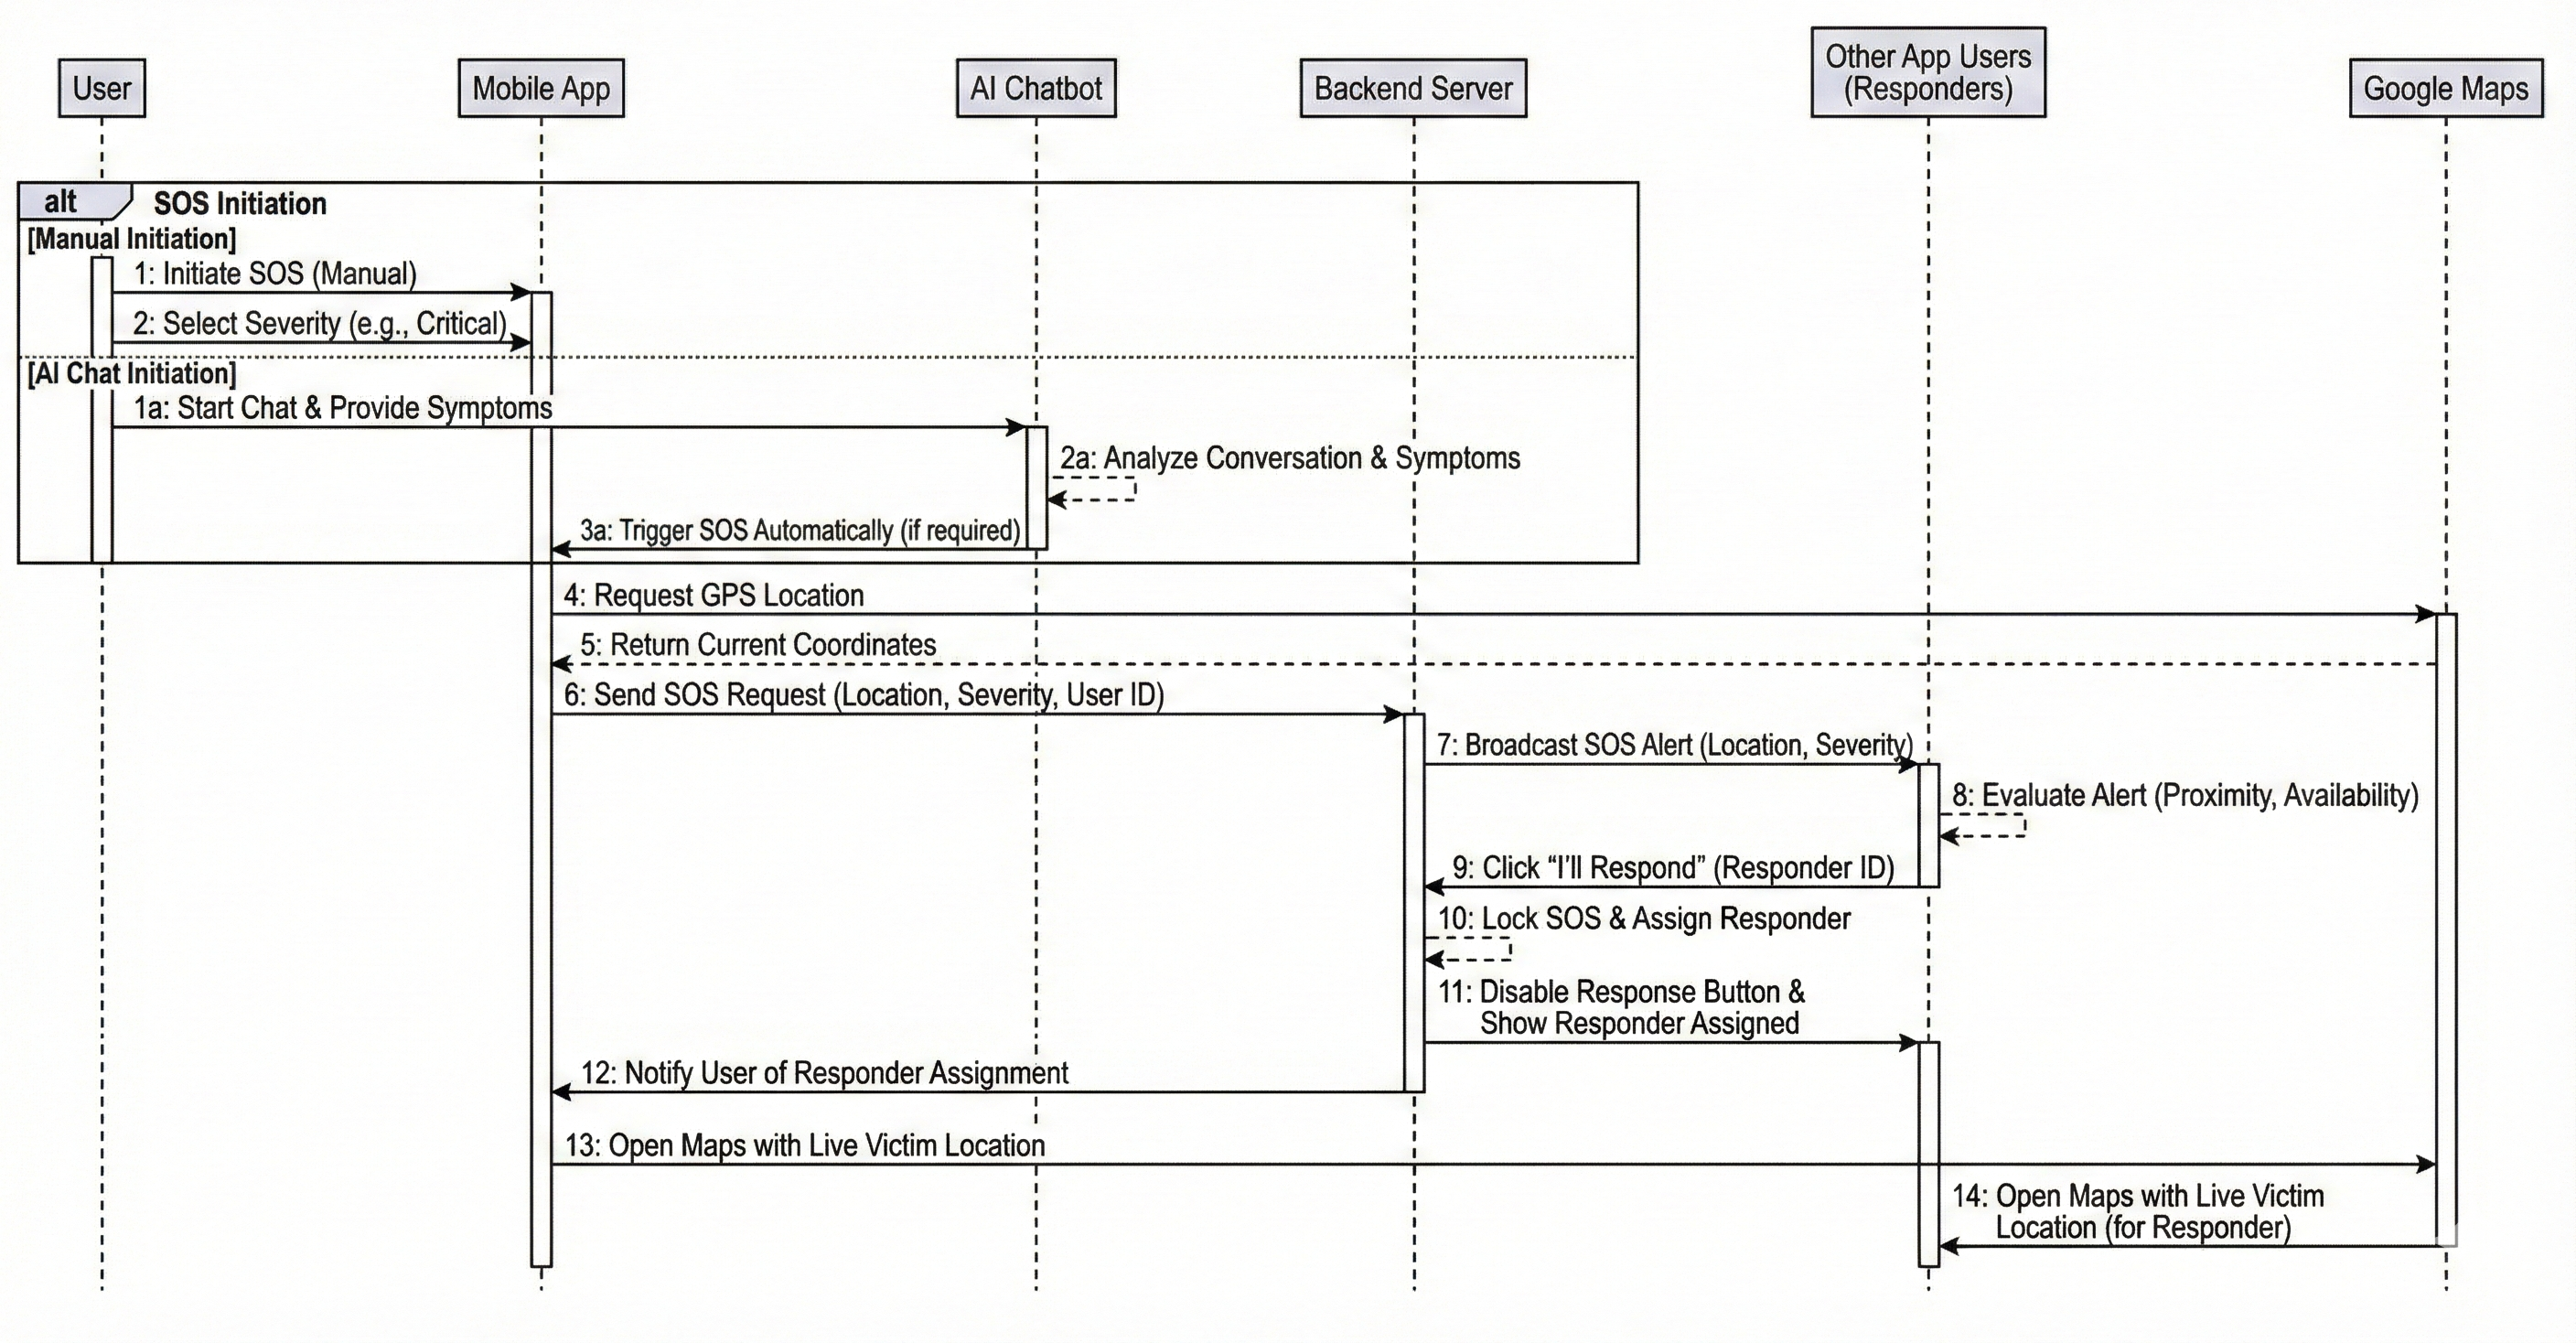
\includegraphics[width=0.95\textwidth]{chapters/complete sos lifecycle sequence in resqnow system.png}
    \caption{Sequence Diagram for Complete SOS Lifecycle in ResQNow System}
    \label{fig:sequence_diagram}
  \end{figure}

  % -----------------------------------------------------------------------------
  \section{Experimental Procedure}

  The experimental evaluation follows a systematic protocol across multiple test scenarios:

  \subsection{Test Scenario 1: SOS Latency Measurement}
  \textbf{Objective:} Measure end-to-end SOS dispatch time under varying network conditions.

  \textbf{Procedure:}
  \begin{enumerate}
    \item Configure test device with timestamp logging enabled
    \item Establish network condition (normal/degraded/poor) using traffic shaping
    \item Press SOS button and record $t_0$
    \item Wait for alert reception on emergency contact device and record $t_6$
    \item Calculate $T_{dispatch} = t_6 - t_0$
    \item Repeat for 30 trials per network condition
    \item Record intermediate timestamps for component-level analysis
  \end{enumerate}

  \subsection{Test Scenario 2: AI Classification Validation}
  \textbf{Objective:} Evaluate classification accuracy against ground truth dataset.

  \textbf{Procedure:}
  \begin{enumerate}
    \item Load prepared test dataset of 100 emergency descriptions
    \item For each test case, submit description to AI classification module
    \item Record predicted emergency type and severity level
    \item Compare prediction with ground truth label
    \item Calculate accuracy, precision, recall, and F1-score
    \item Analyze misclassification patterns and confidence score distributions
  \end{enumerate}

  \subsection{Test Scenario 3: AR Performance Testing}
  \textbf{Objective:} Measure AR initialization latency and rendering performance.

  \textbf{Procedure:}
  \begin{enumerate}
    \item Launch ResQNow application on test device
    \item Trigger AR guidance module and record start timestamp
    \item Measure time to first visual overlay appearance
    \item Monitor frame rate using Android Profiler during 60-second guidance session
    \item Record CPU and GPU utilization
    \item Repeat across 20 trials under consistent environmental conditions
    \item Calculate mean initialization time and average frame rate
  \end{enumerate}

  \subsection{Test Scenario 4: BLE Relay Evaluation}
  \textbf{Objective:} Assess offline message delivery success rate across varying distances.

  \textbf{Procedure:}
  \begin{enumerate}
    \item Position originating device at reference point (0m)
    \item Place relay devices at measured distances: 10m, 30m, 50m, 100m
    \item Position gateway device with internet at 150m from origin
    \item Broadcast 50 test messages from originating device
    \item Record successful deliveries at gateway device
    \item Log RSSI values and hop counts for each message
    \item Calculate success rate as percentage of delivered messages
    \item Repeat experiments with 2, 3, and 5 relay devices
    \item Analyze correlation between distance, node density, and delivery rate
  \end{enumerate}

  \subsection{Test Scenario 5: Resource Utilization Profiling}
  \textbf{Objective:} Quantify battery, network, CPU, and memory consumption.

  \textbf{Procedure:}
  \begin{enumerate}
    \item Charge test device to 100\% battery
    \item Launch Android Battery Historian recording
    \item Execute 1-hour simulated emergency scenario with active GPS, AR, and BLE
    \item Record battery percentage decrease
    \item Use Charles Proxy to capture network traffic during 10 SOS events
    \item Calculate average bandwidth per event
    \item Monitor CPU and memory using Android Profiler during active operations
    \item Record peak and average utilization values
  \end{enumerate}

  % -----------------------------------------------------------------------------

  % -----------------------------------------------------------------------------
  \section{Project Timeline and Development Schedule}

  \subsection{Overview of Development Lifecycle}

  The ResQNow project will be executed following a structured software development lifecycle spanning approximately 11 months from February 2025 to December 2025. The development process will be organized into three major phases: the Planning and Design Phase (February to July 2025) focusing on problem identification, literature review, and system design; the Implementation and Testing Phase (August to November 2025) involving actual development, integration, and validation; and the Documentation and Finalization Phase (November to December 2025) dedicated to report writing and project delivery.

  This timeline allocation ensures adequate time for thorough research, careful design, robust implementation, comprehensive testing, and complete documentation. The extended planning phase is justified by the complexity of integrating multiple advanced technologies including AI, AR, and BLE communication, requiring careful architectural decisions and design validation before implementation begins.

  \subsection{Phase-wise Development Schedule}

  Table~\ref{tab:detailed_timeline} presents the comprehensive project timeline with detailed activities for each development phase. The schedule follows industry-standard software engineering practices with clear milestones and deliverables for each phase.

  \begin{table}[H]
    \centering
    \small
    \caption{Revised Project Development Timeline}
    \label{tab:detailed_timeline}
    \begin{tabular}{|p{3cm}|p{1.8cm}|p{8cm}|}
      \hline
      \textbf{Phase} & \textbf{Duration} & \textbf{Key Activities and Deliverables} \\
      \hline
      \multicolumn{3}{|c|}{\textbf{Planning and Design Phase (4.5 months)}} \\
      \hline
      Background Study & 2 weeks & Research, domain analysis, problem understanding \\
      \hline
      Problem Identification & 2 weeks & Problem formulation, requirement gathering, feasibility study \\
      \hline
      Solution Proposal & 2 weeks & Concept design, technology selection, architecture proposal \\
      \hline
      Literature Review & 3 weeks & Research survey, gap identification, related work analysis \\
      \hline
      Requirements Analysis & 2 weeks & Functional/non-functional requirements, use case modeling \\
      \hline
      System Design & 3 weeks & Architecture planning, DB schema, API specification, UI design \\
      \hline
      UML Modeling & 2 weeks & Use case, activity, sequence, and class diagrams \\
      \hline
      Design Review & 2 weeks & Design validation, feasibility verification, documentation \\
      \hline
      \multicolumn{3}{|c|}{\textbf{Implementation and Testing Phase (4 months)}} \\
      \hline
      Environment Setup & 1 week & Tools installation, Firebase setup, repository initialization \\
      \hline
      Authentication Module & 2 weeks & Login/signup, profile management, Firestore integration \\
      \hline
      GPS and SOS System & 2 weeks & Location tracking, SOS trigger, alert workflow \\
      \hline
      Backend API & 2 weeks & FastAPI configuration, API endpoints, DB operations \\
      \hline
      AI Classification & 2 weeks & Cloud AI integration, rule-based fallback \\
      \hline
      AR Guidance System & 2 weeks & ARCore integration, overlays, CPR/AED guidance \\
      \hline
      BLE Communication & 2 weeks & Offline messaging, encryption, relay testing \\
      \hline
      Notification System & 1 week & Push/SMS/email alerts, multi-channel dispatch \\
      \hline
      System Integration & 2 weeks & Full module integration, workflow validation \\
      \hline
      Performance Testing & 1 week & Latency testing, stress evaluation, optimization \\
      \hline
      \multicolumn{3}{|c|}{\textbf{Documentation and Finalization Phase (2.5 weeks)}} \\
      \hline
      Report Writing & 2 weeks & Technical documentation, diagrams, report draft \\
      \hline
      Final Review & 1 week & Proofreading, formatting, corrections, polishing \\
      \hline
      Submission & 1 day & Final report and presentation submission \\
      \hline
    \end{tabular}
  \end{table}

  \subsection{Gantt Chart Representation}

  Figure~\ref{fig:gantt_chart} presents a Gantt chart visualization of the project timeline showing the duration, sequencing, and overlap of various development activities. The chart provides a clear view of task dependencies and critical path activities that determine the overall project duration.

  \begin{figure}[H]
    \centering
    \includegraphics[width=0.98\textwidth]{chapters/gantt_chart.png}
    \caption{Gantt Chart showing project timeline from February 2025 to February 2026}
    \label{fig:gantt_chart}
  \end{figure}

  The Gantt chart illustrates several important characteristics of the project schedule. The planning phase activities (shown in blue) will execute sequentially with minimal overlap to ensure each design decision is properly informed by previous research. The implementation phase activities (shown in green) will demonstrate higher parallelism where independent modules can be developed concurrently by different team members. The testing activities (shown in orange) will overlap with later implementation tasks to enable early defect detection and continuous quality assurance. The documentation phase (shown in red) will begin while final testing is still underway to maximize efficiency and meet the submission deadline.

  % -----------------------------------------------------------------------------
  \section{Cost Estimation Using COCOMO Model}

\subsection{COCOMO Model Overview}

The Constructive Cost Model (COCOMO) developed by Barry Boehm provides a systematic framework for estimating software development effort, schedule, and cost based on project characteristics. The ResQNow project is estimated using the Basic COCOMO model with adjustments for embedded system characteristics due to mobile and AR components requiring hardware-software integration. The system is classified as \textbf{Semi-Detached mode}, indicating moderate complexity with innovation in technology integration (AI, AR, BLE mesh) while building upon established frameworks (Flutter, Firebase).

\subsection{Project Size Estimation}

Based on functional requirements and architectural design, the ResQNow system size is estimated as follows:

\begin{itemize}
    \item \textbf{Mobile Application Layer:} 8,000 lines of Dart code (UI, state management, device integrations)
    \item \textbf{Backend Services Layer:} 3,000 lines of Python code (API, business logic, database operations)
    \item \textbf{AI Integration Module:} 1,500 lines (API communication, classification, fallback logic)
    \item \textbf{AR Guidance Components:} 2,000 lines (ARCore integration, 3D rendering, overlays)
    \item \textbf{BLE Communication Module:} 1,500 lines (advertising, encryption, relay mechanisms)
\end{itemize}

\textbf{Total Estimated Lines of Code (KLOC):} 16,000 lines = 16 KLOC

\subsection{COCOMO Effort and Schedule Calculation}

Using Basic COCOMO equations for Semi-Detached mode:

\textbf{Effort Calculation:}
\begin{equation}
\text{Effort (E)} = a_b \times (\text{KLOC})^{b_b} = 3.0 \times (16)^{1.12} \approx 60.45 \text{ Person-Months}
\end{equation}

Where $a_b = 3.0$ and $b_b = 1.12$ are COCOMO constants for semi-detached projects.

\textbf{Development Time Calculation:}
\begin{equation}
\text{Development Time (TDEV)} = c_b \times (E)^{d_b} = 2.5 \times (60.45)^{0.35} \approx 10.65 \text{ months}
\end{equation}

Where $c_b = 2.5$ and $d_b = 0.35$ are COCOMO constants.

\textbf{Team Size (Adjusted for 4-Person Team):}
\begin{equation}
\text{Actual Team Size} = 4 \text{ persons}
\end{equation}

\textbf{Adjusted Project Duration:}
\begin{equation}
\text{Adjusted Duration} = \frac{\text{Effort}}{\text{Team Size}} = \frac{60.45}{4} \approx 15.11 \text{ months}
\end{equation}

Since a 4-person team is smaller than the optimal 5.68 persons calculated by COCOMO, the project duration extends from 10.65 to approximately 15 months. However, with efficient task parallelization and agile methodology, the actual duration can be compressed to approximately 11-12 months.

\textbf{Productivity:}
\begin{equation}
\text{Productivity} = \frac{\text{KLOC}}{\text{Effort}} = \frac{16}{60.45} \approx 265 \text{ LOC per Person-Month}
\end{equation}

\subsection{Phase-wise Effort Distribution}

Following the Rational Unified Process (RUP) methodology, effort is distributed across four phases as shown in Table~\ref{tab:phase_effort}.

\begin{table}[H]
\centering
\caption{Phase-wise Effort, Schedule, and Cost Distribution (4-Person Team)}
\label{tab:phase_effort}
\begin{tabular}{|p{2.8cm}|p{2cm}|p{2cm}|p{2.5cm}|p{2.5cm}|}
\hline
\textbf{Phase} & \textbf{Effort (\%)} & \textbf{Effort (PM)} & \textbf{Duration (Months)} & \textbf{Cost (Rs)} \\
\hline
Inception & 6\% & 3.63 & 0.91 & 72,600 \\
\hline
Elaboration & 24\% & 14.51 & 3.63 & 2,90,200 \\
\hline
Construction & 56\% & 33.85 & 8.46 & 6,77,000 \\
\hline
Transition & 14\% & 8.46 & 2.12 & 1,69,200 \\
\hline
\textbf{Total} & \textbf{100\%} & \textbf{60.45} & \textbf{15.12} & \textbf{12,09,000} \\
\hline
\end{tabular}
\end{table}

\textbf{Note:} Duration calculated as Effort (PM) / 4 persons, representing sequential and parallel task execution.

\begin{figure}[H]
    \centering
    \includegraphics[width=0.88\textwidth]{chapters/phase_distribution.png}
    \caption{Phase-wise distribution of effort, schedule, and cost}
    \label{fig:phase_distribution}
\end{figure}

\subsection{Activity-wise Effort Distribution}

Effort distribution across software development activities following industry-standard patterns is shown in Table~\ref{tab:activity_effort}.

\begin{table}[H]
\centering
\caption{Activity-wise Effort Distribution}
\label{tab:activity_effort}
\begin{tabular}{|p{5cm}|p{2.5cm}|p{3cm}|}
\hline
\textbf{Activity} & \textbf{Effort (\%)} & \textbf{Effort (PM)} \\
\hline
Management \& Planning & 10\% & 6.05 \\
\hline
Requirements Analysis & 18\% & 10.88 \\
\hline
Design \& Architecture & 22\% & 13.30 \\
\hline
Implementation (Coding) & 28\% & 16.93 \\
\hline
Testing \& Quality Assurance & 15\% & 9.07 \\
\hline
Documentation & 7\% & 4.23 \\
\hline
\textbf{Total} & \textbf{100\%} & \textbf{60.45} \\
\hline
\end{tabular}
\end{table}

\begin{figure}[H]
    \centering
    \includegraphics[width=0.85\textwidth]{chapters/activity_distribution.png}
    \caption{Activity-wise effort distribution across development tasks}
    \label{fig:activity_distribution}
\end{figure}

\subsection{Detailed Cost Breakdown}

Table~\ref{tab:detailed_cost} provides comprehensive cost breakdown for the ResQNow project with a 4-person development team.

\begin{table}[H]
\centering
\caption{Detailed Project Cost Breakdown (4-Person Team)}
\label{tab:detailed_cost}
\begin{tabular}{|p{4.5cm}|p{5.5cm}|p{2.5cm}|}
\hline
\textbf{Cost Component} & \textbf{Description} & \textbf{Amount (Rs)} \\
\hline
\multicolumn{3}{|c|}{\textbf{Personnel Costs}} \\
\hline
Development Team & 4 developers × 15 months × Rs. 20,000/PM & 12,09,000 \\
\hline
\multicolumn{3}{|c|}{\textbf{Infrastructure \& Services}} \\
\hline
Cloud Services & Firebase, Google Cloud Platform & 15,000 \\
\hline
AI API Usage & OpenAI/Gemini API calls & 20,000 \\
\hline
Communication Services & Twilio SMS, SendGrid Email & 8,000 \\
\hline
\multicolumn{3}{|c|}{\textbf{Hardware \& Testing}} \\
\hline
Testing Devices & Android phones for testing & 25,000 \\
\hline
AR Devices & ARCore-certified devices & 15,000 \\
\hline
\multicolumn{3}{|c|}{\textbf{Documentation \& Miscellaneous}} \\
\hline
Documentation & Report printing, materials & 5,000 \\
\hline
Travel \& Coordination & Team meetings & 3,000 \\
\hline
\multicolumn{3}{|c|}{\textbf{Contingency}} \\
\hline
Risk Buffer (15\%) & Unforeseen expenses & 1,89,000 \\
\hline
\multicolumn{2}{|r|}{\textbf{Total Project Cost}} & \textbf{14,89,000} \\
\hline
\multicolumn{2}{|r|}{\textbf{Rounded Total}} & \textbf{Rs. 15,00,000} \\
\hline
\end{tabular}
\end{table}

\subsection{Cost Distribution Visualization}

Figure~\ref{fig:cost_pie_chart} presents the proportional distribution of costs across major categories, showing that personnel costs constitute approximately 81\% of the total budget.

\begin{figure}[H]
    \centering
    \includegraphics[width=0.82\textwidth]{chapters/cost_pie_chart.png}
    \caption{Percentage distribution of project costs across categories}
    \label{fig:cost_pie_chart}
\end{figure}

The cost breakdown reveals: 81\% personnel costs (labor-intensive development), 5\% infrastructure and services, 3\% hardware and testing, 1\% documentation and miscellaneous, and 13\% contingency reserves for unforeseen circumstances.

\subsection{Risk Factors and Mitigation}

Key risk factors affecting cost estimation:

\begin{itemize}
    \item \textbf{Technology Learning Curve:} AR and BLE expertise development may increase effort by 10-15\%
    \item \textbf{AI API Cost Variability:} Usage costs may vary by 20-30\% based on query volume
    \item \textbf{Integration Complexity:} Multi-technology integration may extend construction by 2-3 weeks
    \item \textbf{Device Compatibility:} Cross-device testing may require additional devices and optimization
    \item \textbf{Scope Changes:} Requirement modifications could increase effort by 10-20\%
\end{itemize}

The 15\% contingency buffer (Rs. 1,89,000) provides risk absorption capacity. Regular sprint reviews and agile adaptation enable proactive risk management within budget constraints.

\subsection{Team Composition and Role Distribution}

The 4-person team structure is organized as follows:

\begin{itemize}
    \item \textbf{Team Lead \& Backend Developer (1):} Project coordination, backend API development, database design, cloud infrastructure management
    \item \textbf{Mobile Developer \& UI/UX (1):} Flutter app development, UI design, state management, GPS integration
    \item \textbf{AI \& AR Specialist (1):} AI classification module, ARCore integration, 3D modeling, computer vision
    \item \textbf{BLE \& Testing Engineer (1):} Bluetooth mesh networking, offline communication, system testing, quality assurance
\end{itemize}

Cross-functional collaboration ensures knowledge sharing and reduces single-point dependencies. Team members contribute to multiple modules based on project phase requirements, enabling efficient resource utilization despite the smaller team size.

\subsection{Conclusion}

The COCOMO-based estimation provides quantitative foundation for planning. With a 4-person team, the project requires 60.45 person-months of effort over approximately 15 months, with an estimated total cost of Rs. 15 lakhs. The phase-wise and activity-wise breakdowns enable effective budget management, milestone tracking, and risk mitigation. While the smaller team size extends the timeline compared to the optimal 6-person configuration, efficient task parallelization, agile methodology, and dedicated role assignments ensure successful delivery of the complex emergency response system integrating AI, AR, and offline communication technologies.
  % -----------------------------------------------------------------------------
  \section{Error Sources and Mitigation Strategies}

  Potential sources of measurement error and corresponding mitigation strategies were identified:

  \subsection{GPS Location Errors}
  \textbf{Error Source:} Indoor environments, urban canyons, and limited satellite visibility degrade GPS accuracy, potentially introducing position errors exceeding 50 meters.

  \textbf{Mitigation:} (1) Implement Kalman filtering for smoothing location coordinates across multiple samples, (2) Use Assisted GPS (A-GPS) leveraging cellular network data for faster satellite lock, (3) Employ Wi-Fi and cellular tower triangulation as fallback positioning methods, (4) Record GPS accuracy estimates provided by location API and flag low-confidence readings, (5) Conduct outdoor testing under clear sky conditions for baseline accuracy establishment.

  \subsection{BLE Signal Propagation Variability}
  \textbf{Error Source:} Physical obstacles (walls, vegetation, terrain), electromagnetic interference from Wi-Fi and other devices, and multipath fading cause unpredictable signal attenuation affecting relay reliability.

  \textbf{Mitigation:} (1) Conduct experiments in open outdoor environments to minimize interference and establish baseline performance, (2) Implement multi-hop relay with acknowledgment-based retries to overcome temporary signal loss, (3) Use message persistence with automatic upload when connectivity is restored, (4) Log RSSI values at each hop to analyze propagation characteristics and identify weak links, (5) Test across multiple device models to account for antenna design variations.

  \subsection{AI Classification Ambiguity}
  \textbf{Error Source:} Vague or incomplete user descriptions, unusual symptom combinations, and rare emergency types may lead to misclassification or low-confidence predictions.

  \textbf{Mitigation:} (1) Implement confidence threshold mechanism triggering rule-based fallback when AI confidence < 0.7, (2) Require user confirmation for moderate-severity classifications before alert dispatch, (3) Provide manual override option allowing users to correct misclassifications, (4) Expand training dataset with diverse emergency scenarios and edge cases, (5) Log misclassification instances for continuous model improvement.

  \subsection{Network Latency Variability}
  \textbf{Error Source:} Network congestion, signal strength fluctuations, and server load variations introduce unpredictable latency affecting response time measurements.

  \textbf{Mitigation:} (1) Conduct multiple trial runs (n=30) per condition to establish statistical distributions and confidence intervals, (2) Implement timeout handling with exponential backoff retry mechanism, (3) Use asynchronous processing to prevent blocking operations, (4) Deploy backend services on auto-scaling infrastructure to handle load spikes, (5) Test across different times of day to capture peak and off-peak network conditions.

  \subsection{Device Hardware Heterogeneity}
  \textbf{Error Source:} Variations in processor speed, GPU capability, RAM capacity, and sensor quality across device models affect AR rendering performance and resource consumption measurements.

  \textbf{Mitigation:} (1) Test on representative device models spanning low-end, mid-range, and high-end hardware configurations, (2) Implement device capability detection with adaptive quality settings for AR rendering, (3) Provide graceful degradation fallback to non-AR guidance on incompatible devices, (4) Normalize performance metrics by device specifications when comparing results, (5) Document minimum hardware requirements for optimal system operation.

  \subsection{Timestamp Synchronization Errors}
  \textbf{Error Source:} Clock drift between client devices and servers, network propagation delay in timestamp transmission, and timezone inconsistencies may introduce timing measurement inaccuracies.

  \textbf{Mitigation:} (1) Synchronize device clocks with Network Time Protocol (NTP) servers before measurement sessions, (2) Use high-precision system clocks with microsecond resolution (SystemClock.elapsedRealtimeNanos() on Android), (3) Calculate latency components using same-device timestamps where possible to eliminate synchronization errors, (4) Record UTC timestamps to avoid timezone conversion issues, (5) Validate timestamp consistency by comparing calculated latencies against expected ranges.

  % -----------------------------------------------------------------------------
  \section{Data Analysis Methodology}

  Collected experimental data undergoes systematic statistical analysis to validate system performance and identify optimization opportunities:

  \subsection{Descriptive Statistics}
  For each measured parameter, calculate:
  \begin{itemize}
    \item \textbf{Mean ($\mu$):} Average value across all trials
    \item \textbf{Standard Deviation ($\sigma$):} Measure of variability
    \item \textbf{Minimum and Maximum:} Range of observed values
    \item \textbf{95\% Confidence Interval:} Statistical reliability bounds
  \end{itemize}

  \subsection{Comparative Analysis}
  Compare system performance across conditions using:
  \begin{itemize}
    \item \textbf{Latency comparison graphs:} Bar charts showing $T_{dispatch}$ under normal, degraded, and poor network conditions
    \item \textbf{Classification accuracy tables:} Confusion matrices comparing predicted vs. actual emergency types
    \item \textbf{BLE success rate plots:} Line graphs showing delivery rate as function of distance and node density
    \item \textbf{Resource utilization charts:} Stacked bar graphs comparing battery, CPU, and memory consumption across scenarios
  \end{itemize}

  \subsection{Statistical Validation}
  Apply statistical tests to validate performance claims:
  \begin{itemize}
    \item \textbf{Hypothesis testing:} Verify if $T_{dispatch}$ meets target threshold ($< 3000$ ms) with statistical significance
    \item \textbf{Correlation analysis:} Examine relationships between distance and BLE success rate, network quality and latency
    \item \textbf{Regression analysis:} Model performance trends and predict behavior under untested conditions
  \end{itemize}

  \subsection{Visualization Techniques}
  Present results using:
  \begin{itemize}
    \item Box plots showing latency distributions and outliers
    \item Scatter plots correlating GPS accuracy with environmental factors
    \item Heat maps visualizing classification confusion matrices
    \item Time series graphs tracking resource consumption over duration
  \end{itemize}

  All graphs and tables are prepared using Python libraries including Matplotlib, Seaborn, and Pandas for reproducible analysis. Raw measurement data is archived in CSV format for future reference and verification.

  % -----------------------------------------------------------------------------
}
